
%\begin{center}
%\Large\textbf{Short-Baseline Neutrino Program}
%\end{center}

\begin{center}
\textbf{ \Large{Executive Summary} }
\end{center}

The Intensity Frontier (I.F.) group of the University of Texas at Arlington started in 2014 with 0.5 FTE of PI Jae Yu and PI Amir Farbin aiming for a balanced program between US-based and non-US based experiments. In order to continue to build a strong I.F. program, the group recently hired full time I.F. junior faculty, Dr. Jonathan Asaadi. While PI Farbin has decided to transition back to the Energy Frontier (E.F), the overall strength of the group has grown to two FTE with the successful transition of PI Yu to full time I.F.

Beyond the addition of a new faculty member, the UTA I.F. group has made significant contributions to the LArIAT, LBNE/DUNE, and MiniBooNE Experiments. Farbin played a key role of computing coordinator for the DUNE project and Yu has served as a co-convener for the LBNE R$\&$D Coordination group. This role has now become a co-convenership of the DUNE Beyond the Standard Model physics group since September 2015. UTA was also the host of the DUNE collaboration meeting in January, 2016, in which over 150 collaborators participated. Asaadi has continued his roles on MicroBooNE, serving as convener of the Astro-Particle and Exotics group through August 2016 and lead TPC-Expert for the experiment. Asaadi has also played a leadership role on LArIAT serving as the analysis coordinator and now to serve as co-spokesperson (starting Fall 2016). The UTA group has also joined SBND (through Asaadi's existing affiliation) and the ICARUS experiment (with Yu as institutional board member) and have been contributing to the refurbishment of the light detection system with the hire of a new post-doctoral researcher (and existing ICARUS collaborator), Dr. Andrea Falcone.

In this document, we propose to complete the ongoing effort on MiniBooNE (Yu), and continue/add significant contributions to SBND (Asaadi, Yu), MicroBooNE (Asaadi), ICARUS (Asaadi, Yu) and the Deep Underground Neutrino Experiment, DUNE (Asaadi, Yu) with a vital contribution to protoDUNE. These experiments are carefully selected to leverage our groups growing technical and analysis expertise utilizing liquid argon time projection chambers. Moreover, in order to accomplish the work laid out in this proposal, the UTA group will leverage Asaadi's start-up to provide an additional (beyond what is requested here) post-doctoral researcher (Dr. Andrea Falcone) in year one and two of this propsal. Dr. Falcone will play a leadership role on the ICARUS and SBND experiments during construction, installation and commissioning.

The work on MiniBooNE is limited to data analysis from the beam dump data taken in 2014 for a low mass dark matter search. This is anticipated to complete shortly with the graduation of Sepideh Shahsavarani, Farbin’s Ph.D. student. This student will stay on the I.F. program for another two years till she completes her Ph.D. under the joint advisement of Farbin, Yu, and Asaadi. We anticipate the data taking and analysis work we have been involved in LArIAT will conclude as the experiment completes within the next 1-2 year time scale. 
 

%Yu applied for a sabbatical leave and stayed at CERN from late September 2015 through mid May, 2016, during which time he had contributed to WA105 small ($3\times 1 \times 1~{\rm m^{3}}$) prototype construction and understanding the behavior of the membrane cryostat.


\subsubsection{Introduction}
The discovery that neutrinos undergo oscillation in their flavor, and thus are massive particles, serves as one of the first pieces of evidence for physics beyond the Standard Model (SM) of particle physics. The prevailing description of neutrino oscillations provided by the Pontecorvo-Maki-Nakagawa-Sakata (PMNS) matrix characterizes the flavor change as a result that the neutrino flavor eigenstates ($\nu_{e}, \nu_{\mu}, \nu_{\tau}$) are a linear combination of the neutrino mass eigenstates ($\nu_{1}, \nu_{2}, \nu_{3}$). The rotation from the mass eigenstates to the flavor eigenstates is governed by three angles $\theta_{i,j}$, where $i$ and $j$ correspond to the mass eigenstates with $i < j$, and a phase $\delta$ which determines magnitude of charge-parity (CP) violation within the neutrino sector. Additionally, the flavor change of the neutrinos depends on the ratio neutrino energy and the distance traveled by the neutrino (often referred to as the baseline) as well as the difference in the square of the mass eigenstates $\Delta m_{ji}^{2}$. Neutrinos produced in the atmosphere \cite{No1, No2, No3}, in nuclear reactors \cite{No4, No5, No6}, in the sun \cite{No7, No8, No9}, as well as in man-made particle accelerators \cite{No10, No11, No12} have been used to study the phenomenon of neutrino oscillations. The exact ordering of the neutrino mass states, known as the mass hierarchy, as well as the size of the CP-violating phase $\delta$ are, as yet, unknown. These quantities remain one of the last major pieces of the Standard Model of particle physics and offer the opportunity to answer such fundamental questions as:

\begin{itemize}
\item[1)] \textbf{What is the origin of the matter/antimatter asymmetry in the universe?}

\item[2)] \textbf{Do we understand the fundamental symmetries of the universe?}

\item[3)] \textbf{Is the three-flavor paradigm of the Standard Model for neutrino oscillation the accurate description for neutrino interactions?}
\end{itemize}

Into this experimental landscape, there exists a set of series of experimental measurements which suggest that the three-flavor paradigm of neutrino oscillations is incomplete. Two general classes of anomalous observations may point to additional physics beyond the SM  in the neutrino sector.

\begin{itemize}
\item \textbf{The disappearance signal in low energy electron anti-neutrinos from reactor neutrino experiments \cite{No13} \textit{(``Reactor Neutrino Anomaly'')} and Mega-Curie radioactive electron neutrino sources in Gallium \cite{No14, No15} \textit{(``Gallium Anomaly'')}}

\item \textbf{The electron-like excess from muon neutrino (and anti-neutrino) particle accelerators \textit{(``LSND/MiniBooNE Anomaly'')} \cite{No16, No17}}

\end{itemize}

Neither of these anomalies can be accounted for by the standard three-flavor oscillations of the SM and may hint at the existence of additional neutrino states with larger mass difference ($\Delta m_{new}^{2}\geq 0.1 eV^{2}$) which participate in the mixing of the flavour states (referred to as ``sterile neutrinos''). Definitive evidence of the existence of new neutrino states would be a revolutionary discovery with broad implications for both particle physics and cosmology. Moreover, in order for future accelerator based neutrino experiments to disentangle the mass hierarchy and search for CP-violation, the oscillation framework must be concretely known and precisely measured.

Liquid Argon Time Projection Chambers (LArTPCs) offer fine-grain tracking as well as powerful calorimetry and particle identification capabilities making them ideal detectors for studying neutrino-nuclei interactions. When a neutrino interacts with an atom in the liquid argon multiple final state charged particles as well as electromagnetic objects (such as photons and electrons) can be produced. When the charged particles traverse the liquid argon they produce ionization which drifts along the electric field inside the TPC towards a set of wire planes which are oriented at different angles with respect to each other. The drifting ions produce an electric signal on the wire planes, which is read out of the detector. By knowing the drift speed of the ions and the timing of the interaction as well as the deposition of charge on the wires a three-dimensional image of the interaction can be reconstructed. The information of the charge deposition in addition to the topological information allows for particle identification and calorimetric reconstruction. This allows, for example, the ability to disentangle electron initiated electromagnetic showers from photon initiated showers by looking at the displacement in the start of the electromagnetic shower from a primary vertex as well as analysing the energy deposited in the first centimetres of the shower (dE/dX), shown schematically in Fig. \ref{fig:LArTPC}.

\begin{figure}[htb]
\centering
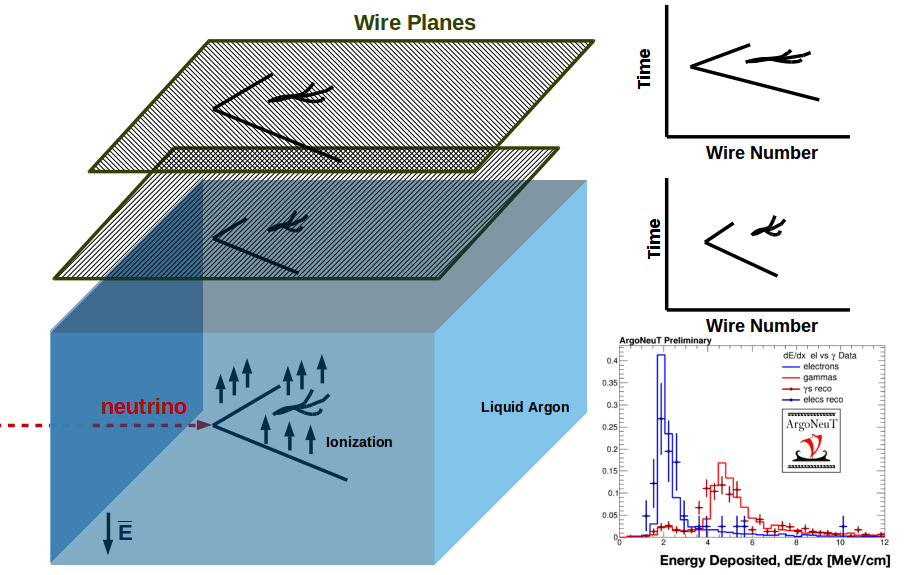
\includegraphics[width=0.55\textwidth]{images/lartpc.png}
\caption[]{Operating principals of LArTPC detectors.}
\label{fig:LArTPC}
\end{figure}

For these reasons, this detector technology has been chosen for both the study of neutrino oscillations over relatively short baselines ($<1$~km) and long baselines ($>1000$~km). The combination of millimeter scale tracking capabilities, outstanding calorimetry through a fully active/sampling detector, and powerful particle identification made by combining the ionization along the particle trajectory (dE/dX) and the topological information, have made LArTPCs the premier neutrino detector technology choice for the future. 

The UTA intensity frontier group has grown recently with the addition of a junior faculty member, Jonathan Asaadi,and the complete transition of senior faculty Jaehoon Yu to the intensity frontier effort. The UTA group will have contributions and responsibilities across the Fermilab the short-baseline neutrino (SBN) program as well as the long-baseline neutrino (LBN) program. A summary of the experiments, projects and PI's responsibilities is provided in Table \ref{tab:IFProjects}. The details of these projects are given in the subsequent sections.

\begin{center}
\begin{table}[htb]
	\begin{center}
	\resizebox{0.95\textwidth}{!}{%
	\begin{tabular}{c|c|c|c}
	\multicolumn{4}{c}{\textbf{IF Summary of Proposed Work}} \\
	\hline \hline
	\textbf{Experiment} & \textbf{Project} & \textbf{Description} & \textbf{Lead PI} \\
	\hline
	     & Vertical Slice Test-Stand & Say things here & Asaadi \\
    SBND & Detector Construction, Installation, and Commissioning & Details & Yu \\	     
	     & High-statistics cross-section & Details & Asaadi \\
	     
	\hline
	MicroBooNE & TPC Detector Expert & Say things here & Asaadi \\
	           & Coherent Charged Pion Cross-Section & Details & Asaadi \\
	\hline
	ICARUS     & Detector Installation and Commissioning & Details & Asaadi \\
	           & NuMI Off-Axis Cross-Sections & Details & Yu \\
	           
	\hline
	     & protoDUNE Single Phase APA QA/QC and installation & Details & Asaadi \\
	DUNE & BSM Physics & Details & Yu \\
	     & protoDUNE Dual Phase FC Construction & details & Yu \\
	\hline
	MiniBooNE & Beam Dump Dark Matter Search & details & Yu \\
	\hline                      
	\end{tabular}}
	\caption{Overview of the UTA projects across the Intensity Frontier} \label{tab:IFProjects}
	\end{center}
\end{table}
\end{center}


 
 
 DUNE (Asaadi, Yu) aims to address the questions of the neutrino mass hierarchy and CP-violation in the lepton sector. The SBN program aims to conclusively address the experimental hints of sterile neutrinos through the utilization of three LArTPC detectors: the Short-Baseline Near Detector (SBND) (Asaadi, Yu), the Micro-Booster Neutrino Experiment (Asaadi), and the ICARUS Experiment (Asaadi, Yu). All three of these SBN experiments as well as DUNE are strategically selected to leverage the UTA expertise in LArTPC technology across them.
Asaadi is playing a leading role in the operations of MicroBooNE experiment. Asaadi and Yu will play key roles in the construction, commissioning, and operation of SBND through contributions to cold electronics testing, APA assembly, and operations of the detector. These efforts build on our experience in commissioning of the LArIAT and MicroBooNE experiments. UTA is actively involved in the ICARUS experiment where Yu is currently the IB representative and a post-doc is helping the refurbishment of the light detectors at CERN.  UTA is also playing key roles in the construction of protoDUNE detectors, template DUNE far detectors. Asaadi is involved in quality assurance and construction of the single phase (SP) protoDUNE. Yu is leading the DUNE BSM physics group and is involved in design and construction of dual phase protoDUNE field cage whose design shares large portion of the SP protoDUNE field cage. These activities aim to ensure synergy between the SBN and LBN efforts and an optimized use of resources.



